\documentclass[12pt,a4paper]{article}
\usepackage[utf8]{inputenc} % sempre salve seus arquivos como UTF8
\usepackage[T1]{fontenc}
\usepackage[english]{babel}

\usepackage[left=2.5cm,right=2cm,top=2cm,bottom=2.5cm]{geometry}
\usepackage{amsmath}
\usepackage{amsthm}
\usepackage{amsfonts}

\usepackage{graphicx}
\usepackage{algorithm}
\usepackage{color}
\usepackage[noend]{algpseudocode}
\usepackage{mathtools}
\usepackage{subfig}
\usepackage{diagbox}

% load times font
\usepackage{mathptmx}
\usepackage[scaled=.90]{helvet}
\usepackage{courier}

% comandos
\newcommand{\mdc}[1]{\mathrm{mdc}(#1)}

\DeclarePairedDelimiter\ceil{\lceil}{\rceil}
\DeclarePairedDelimiter\floor{\lfloor}{\rfloor}

% Foot without marker
\newcommand\blfootnote[1]{%
	\begingroup
	\renewcommand\thefootnote{}\footnote{#1}%
	\addtocounter{footnote}{-1}%
	\endgroup
}

\title{MO446 -- Introduction to Computer Vision  \\ Project 1}
\author{Breno Leite  \\ Guilherme Leite}
\date{28/08/2017}

\begin{document}

\maketitle
\blfootnote{\textit{\textbf{Important note:} The borders seen in the figures are not part of the image, they are figurative information about the starting and ending points of the image. Moreover, all the image scales in this report were changed in order to make the text more readable.}} \\

%% ---------------- Starts here --------------------------------

\textbf{\LARGE Input Images}\\

Throughout this project some images were used as input to test the algorithms. Figure \ref{fig:p1-1-0} was used as input for the pyramids exercises \textbf{2.1, 2.2, 2.3} and \textbf{3.1}, its dimensions are 400x300 and it is a colored image. \\

\begin{figure}[!h]
	\centering
	{%
		\setlength{\fboxsep}{1pt}%
		\setlength{\fboxrule}{1pt}%
		\fbox{
\includegraphics[scale=1]{input/p1-1-0}}%
	}%
	\caption{Input image for pyramids and fourier transform exercices. (\textbf{p1-1-0})}
	\label{fig:p1-1-0}
\end{figure}

\newpage

The Figures in \ref{fig:blending} are used for the blending exercises (\textbf{2.4} and \textbf{3.2}), all of them have dimensions 540x392 and are colored. Note that the images are slightly rotated, this will affect some results which comes from the image and not by any error on the process itself. \\

\begin{figure}[!h]
	\centering
	\subfloat[Image 1 (\textbf{p1-2-4-0})]{
		{
			\setlength{\fboxsep}{1pt}
			\setlength{\fboxrule}{1pt}
			\fbox{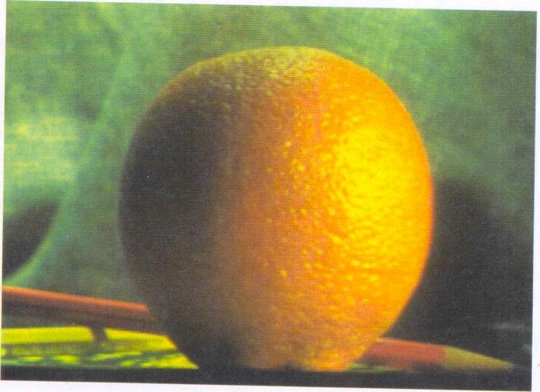
\includegraphics[scale=0.75]{input/p1-2-4-0}}
		}
	}
	\quad
	\subfloat[Image 2 (\textbf{p1-2-4-1})]{
		{
			\setlength{\fboxsep}{1pt}
			\setlength{\fboxrule}{1pt}
			\fbox{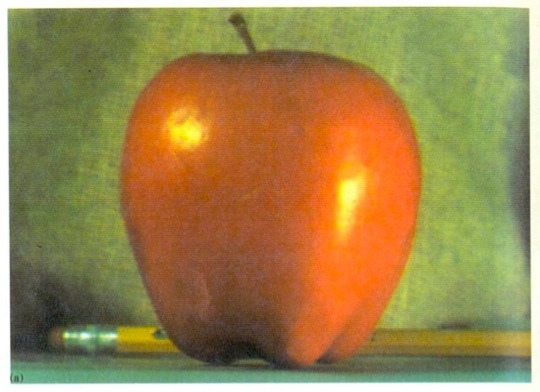
\includegraphics[scale=0.75]{input/p1-2-4-1}}
		}
	}
	\caption{Images 1 and 2 used for the blending operations.}
	\label{fig:blending}
\end{figure}

\textbf{\LARGE Question 2 - Spatial blending}\\

\textbf{2.1 )} In the spectrum of image processing, convolution can be understood as the action of applying a mask to an image, in this case every pixel in the image is affected by the weighted sum of the filter applied to the pixel neighborhood. This approach requires some special attention when dealing with the edges of the image, since the application of the mask will overshoot the image borders, our solution to this problem was to extend the original image filling it's new borders with zeros, as seen in Figure \ref{fig:make-border}, by doing so the convolution simply ignore those values and don't account them into the result, a minor downside to this approach is the lessen effect of the mask around the edges, this solution was chosen for it's simplicity to implement. Additionally the convolution was tested with three smoothing masks, 3x3, 7x7 and 15x15, in comparison to the embedded solution by OpenCV our convolution was noticeably slower as seen in Table \ref{table:convolution-opencv}. As expected the masks smooth the edges around the image and suffers with a darkening close to the borders as seeing in Figure \ref{fig:p1-2-1-0}, with bigger masks the image suffered more distortion to the point of loosing all of its fine details, see Figure \ref{fig:p1-2-1-2}, the loss of such details is accounted by the size of the neighborhood that affect each pixel, thus a larger mask smooths more than a smaller one.\\

\begin{figure}[!h]
	\centering
	{%
		\setlength{\fboxsep}{1pt}%
		\setlength{\fboxrule}{1pt}%
		\fbox{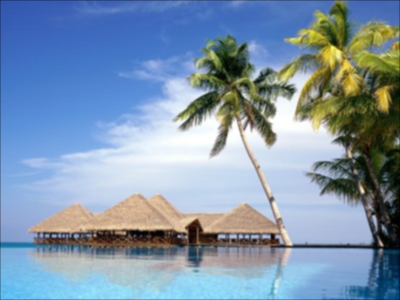
\includegraphics[scale=0.7]{output/p1-2-1-0}}%
	}%
	\caption{Convolution with 3x3 mask (\textbf{p1-2-1-0})}
	\label{fig:p1-2-1-0}
\end{figure}

\begin{figure}[!h]
	\centering
	{%
		\setlength{\fboxsep}{1pt}%
		\setlength{\fboxrule}{1pt}%
		\fbox{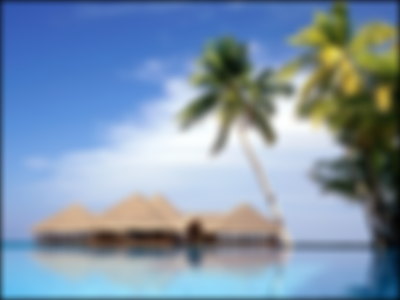
\includegraphics[scale=0.7]{output/p1-2-1-2}}%
	}%
	\caption{Convolution with 15x15 mask (\textbf{p1-2-1-2})}
	\label{fig:p1-2-1-2}
\end{figure}

\begin{table}[!h]
 \centering
 \begin{tabular}{|c|c|c|c|}
	\hline
		& \multicolumn{3}{c|}{\textbf{Time (ms)}} \\ \hline
		\backslashbox{\textbf{Convolution}}{\textbf{Mask Size}}    & \textbf{3x3}         & \textbf{7x7}          & \textbf{15x15}      \\ \hline
	\textbf{Implemented}  & 5.123      & 4.8681      & 5.238     \\ \hline
	\textbf{OpenCV} & 0.006      & 0.004       & 0.019     \\ \hline
	\end{tabular}
 \caption{Comparission of time between our implementation and OpenCV convolution.}
 \label{table:convolution-opencv}
 \end{table}

\textbf{2.2 )} To store the gaussian and laplacian pyramids of this project we chose a list, in which each node of it holds a level of the pyramid. Since the data structure is a list the access method is as in a array, $pyramid[i]$ returns the image in the ith pyramid level, disregarding then, the necessity to implement an access function. The strategy chosen to implement the interpolation was the bilinear interpolation. These decisions were taken regarding the time to implement and simplicity to understand. It is also worth noting that due to some confusion about the meaning of Up and Down, these functions were renamed as follow: Expand referring to the action of expand the image width and height, and Contract analogously. Figure \ref{fig:guassianPyramid} shows the pyramid formed with the implemented function. \\

\textbf{2.3 )} The laplacian pyramid demanded more attention to it's details, such as the fact that the last level of the pyramid is a copy of the same level at the gaussian pyramid. This particular level is used to perform the reconstruction of the original image, first the image is extended and interpolated, to match the previous level size, then it is summed with the previous level of the pyramid, the repetition of these steps result in the original image that was compressed in the pyramid, Figure \ref{fig:placePyramid} shows the laplacian pyramid. \\

\textbf{2.4 )} In this exercise the blending was achieved by the following steps:

Starting at the top of the laplacian pyramid
Apply the mask and its negative to each image
blend the images and reconstruct the previous pyramid level
repeat

\newpage

\textbf{\LARGE Question 3 - Frequency Blending} \\

In this question, we will present some experiments developed using \emph{numpy} and \emph{OpenCV} function in order to transform the image from the spatial domain to the frequency domain. The process will be divided into two different experiments. \\

On the first one (\textbf{3.1}), we will use the transformation and make some modifications to the phase and magnitude in order to see the impact on the image recontructed. On the second experiment (\textbf{3.2}), we will be blending the two images used into the question \textbf{4.2} in order to check how it is compared to the spatial blending. \\

\textbf{3.1 )} Exploring Fourier Space \\

In order to explore the fourier space, we implemented two functions. One to transform an image into magnitude and phase, and the other to reconstruct the image from magnitude and phase. The Figure \ref{fig:mag-phase} shows the magnitude and phase obtained transforming the Figure \ref{fig:p0-1-0} to the frequency domain. \\

\begin{figure}[!h]
	\centering
	\subfloat[Phase Image (\textbf{p1-3-1-0})]{
		{
			\setlength{\fboxsep}{1pt}
			\setlength{\fboxrule}{1pt}
			\fbox{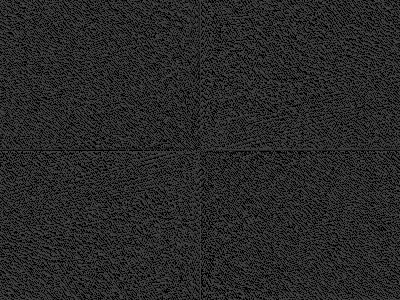
\includegraphics[scale=0.5]{output/p1-3-1-0}}
		}
		\label{fig:phase}
	}
	\quad
	\subfloat[Magnitude Image (\textbf{p1-3-1-1})]{
		{
			\setlength{\fboxsep}{1pt}
			\setlength{\fboxrule}{1pt}
			\fbox{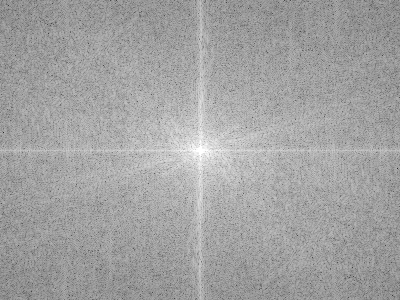
\includegraphics[scale=0.5]{output/p1-3-1-1}}
		}
		\label{fig:magnitude}
	}
	\caption{Phase and Magnitude images created on the fourier transform using image \textbf{p0-1-0}.}
	\label{fig:mag-phase}
\end{figure}

In order to create these images, the results of the fourier transform were shifted to the center and then reduced by the functions, $20*log_e(magnitude)$ and $40*log_e(phase)$. These values were used to mantain the values between 0 and 255, which could be showed as an image. These values are translated back when doing the reverse of the fourier transform. \\

The Figure \ref{fig:phase} shows the phase of the image, it is hard to obtain some information from this image. However, it is respective to the directions of the image. Moreover, the Figure \ref{fig:fig:magnitude} shows the values to the magnitude, the intensity shows the values of the magnitude. In both Figures, light pixels indicates high values.

We can have a little more information with the magnitude image, it is noticeably that the image is bright, which indicates that the image on Figure \ref{fig:p0-1-0} has more high frequency than low frequency. \\



\textbf{3.2 )} Blending \\

\end{document}
